\section{Debriefing ed esiti dell'esperimento}
Lo scopo di questo paragrafo � quello di analizzare i dati raccolti dall'esperimento con l'utente ed esplicitarne gli esiti. Nelle varie analisi i dati verranno mostrati suddivisi per categoria di utente (che ricordiamo aver definito come ``esperti'' e ``non esperti'') in un unico grafico, per mostrare meglio le differenze nei tempi in cui vengono portati a termine i compiti, a seconda delle categorie di utenti.
\subsection*{Giudizio espresso dall'utente}
Grafico riguardante la valutazione degli utenti in riferimento ai vari task, nel seguente grafico (figura:\ref{fig:grafico_difficolta}) sono mostrate le valutazioni medie di difficolt�, utilizzando i seguenti valori come pesi: banale 0; facile 1; medio 2; impegnativo 3; difficile 4.
\begin{figure}[!h]
\centering
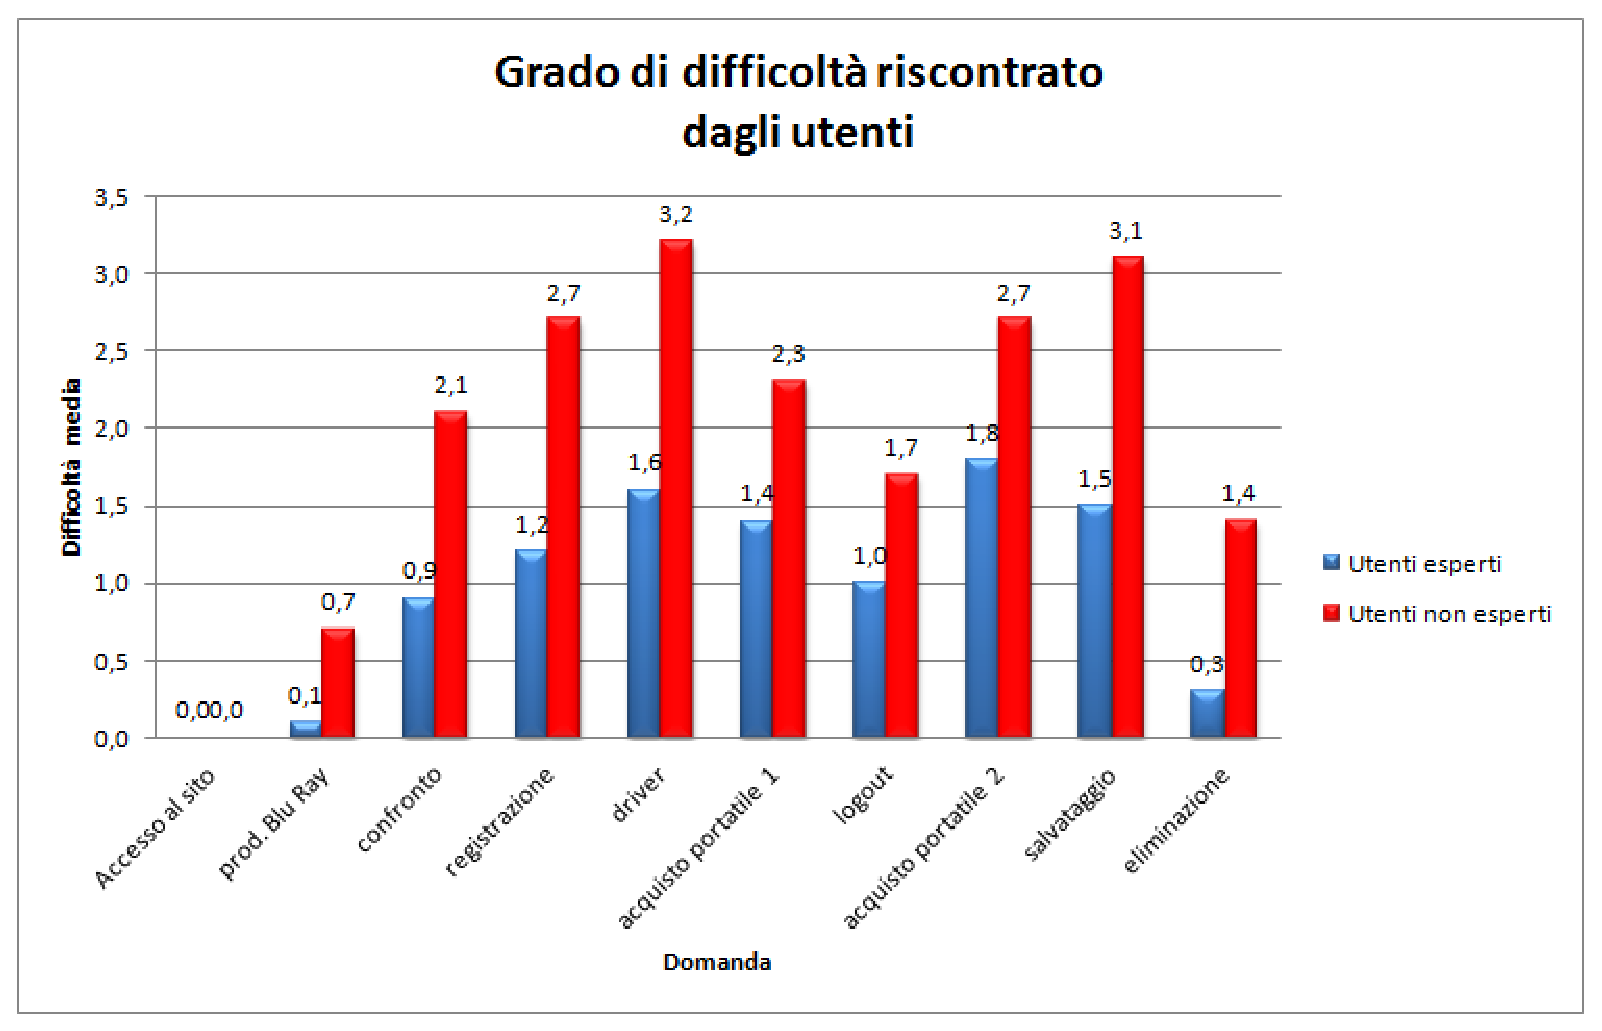
\includegraphics[angle=90,scale=0.75]{figure/grafico_difficolta.eps}
\caption{Grafico media delle difficolt� dei due gruppi d'utenti esaminati}
\label{fig:grafico_difficolta}
\end{figure}
Come evidenziato dal grafico gli utenti esperti considerano i compiti a loro assegnato notevolmente pi� semplici dei loro corrispettivi non esperti. In particolare si evidenzia che la fase di registrazione e di salvataggio della configurazione del secondo portatile risultano avere una valutazione di difficolt� pi� che doppia. Si nota inoltre che alcuni compiti che dovrebbero risultare semplici in realt� non siano tali, come ad esempio la registrazione ed il salvataggio delle proprie impostazioni. Inoltre alcuni utenti hanno valutato la difficolt� di compiti da loro eseguiti fuori tempo massimo o in maniera errata come facile o media.

\subsection*{Valutazione di tempi ed errori}
Esponiamo ora i dati oggettivi raccolti dai due valutatori ossia il tempo impiegato per risolvere i vari task, e gli errori riscontrati per ogni singolo task. Nei seguenti diagrammi si � deciso di mantenere i dati di utenti esperti e non esperti separati, come abbiamo fatto nel paragrafo precedente.


\begin{figure}[!h]
\centering
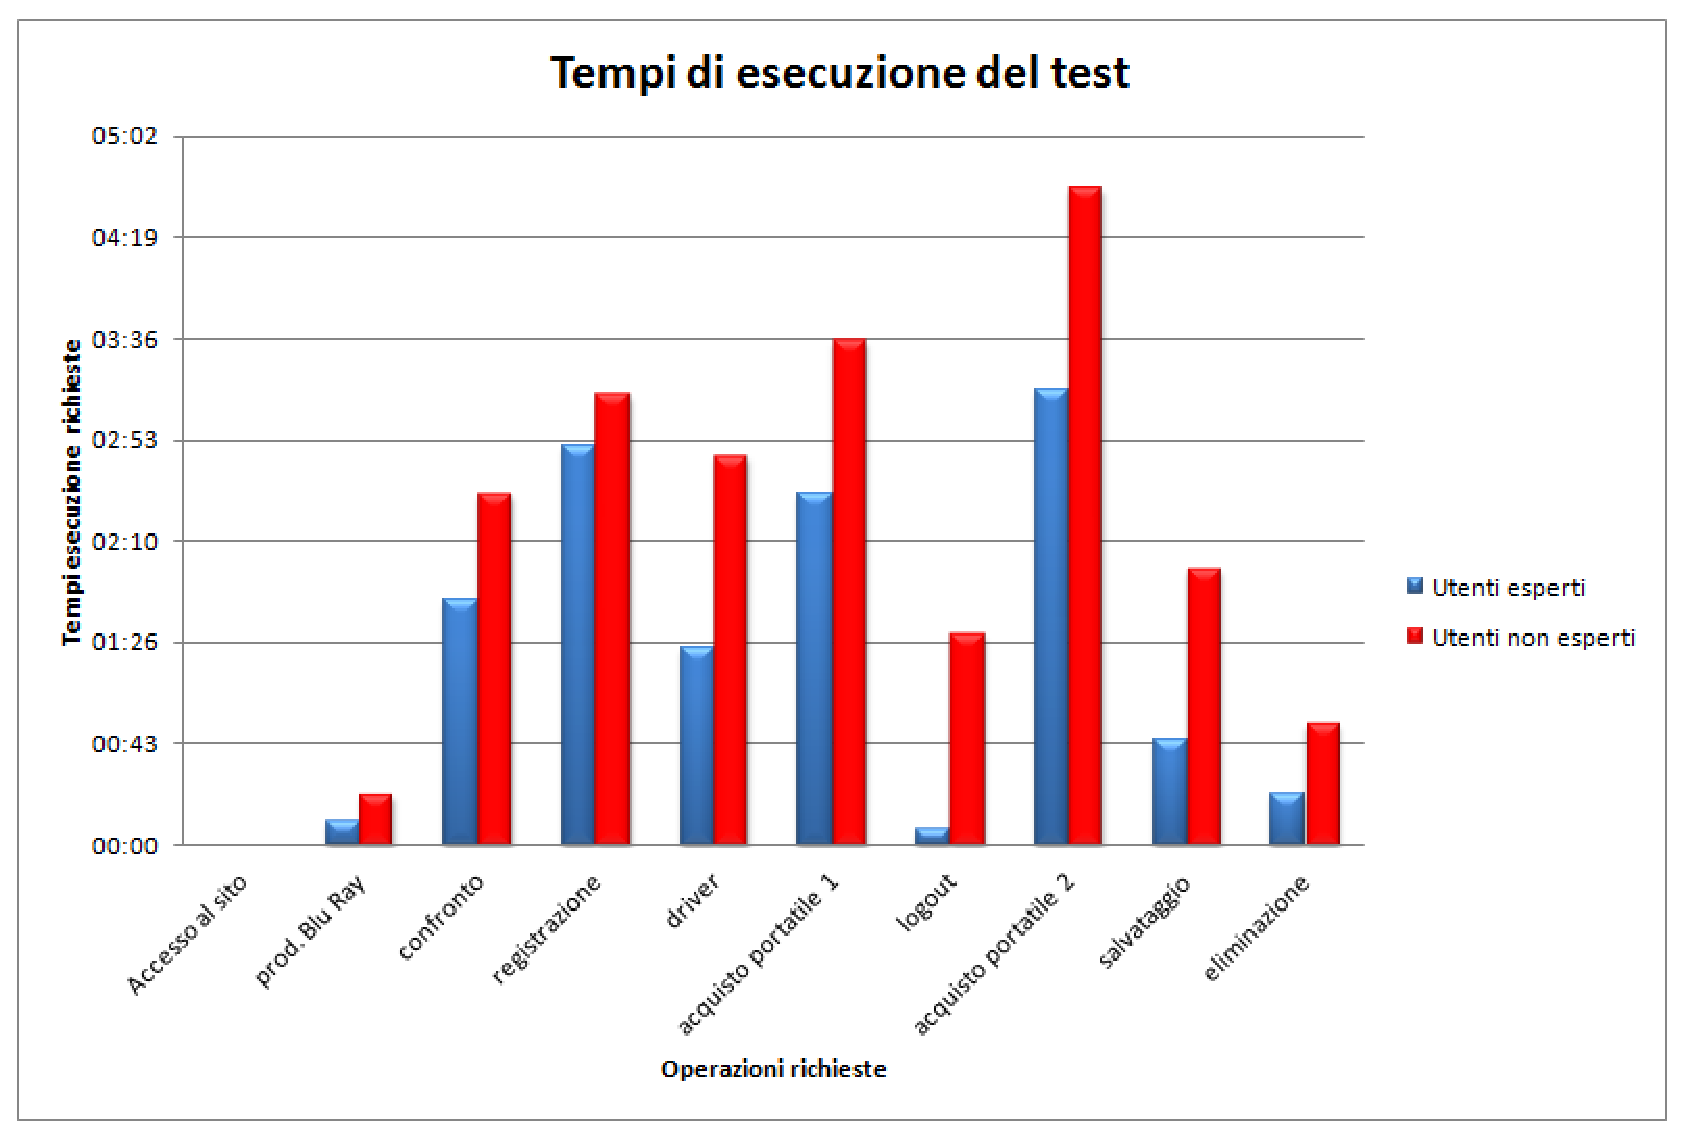
\includegraphics[angle=90, scale=0.75]{figure/grafico_tempi_esecuzione.eps}
\caption{Grafico riportante i tempi di esecuzione delle varie domande del test}
\label{fig:tempi_esecuzione_test}
\end{figure}

Dopo il grafico riguardante i tempi medi passiamo a vedere quello riguardante la quantit� di errori:

\begin{figure}[!h]
\centering
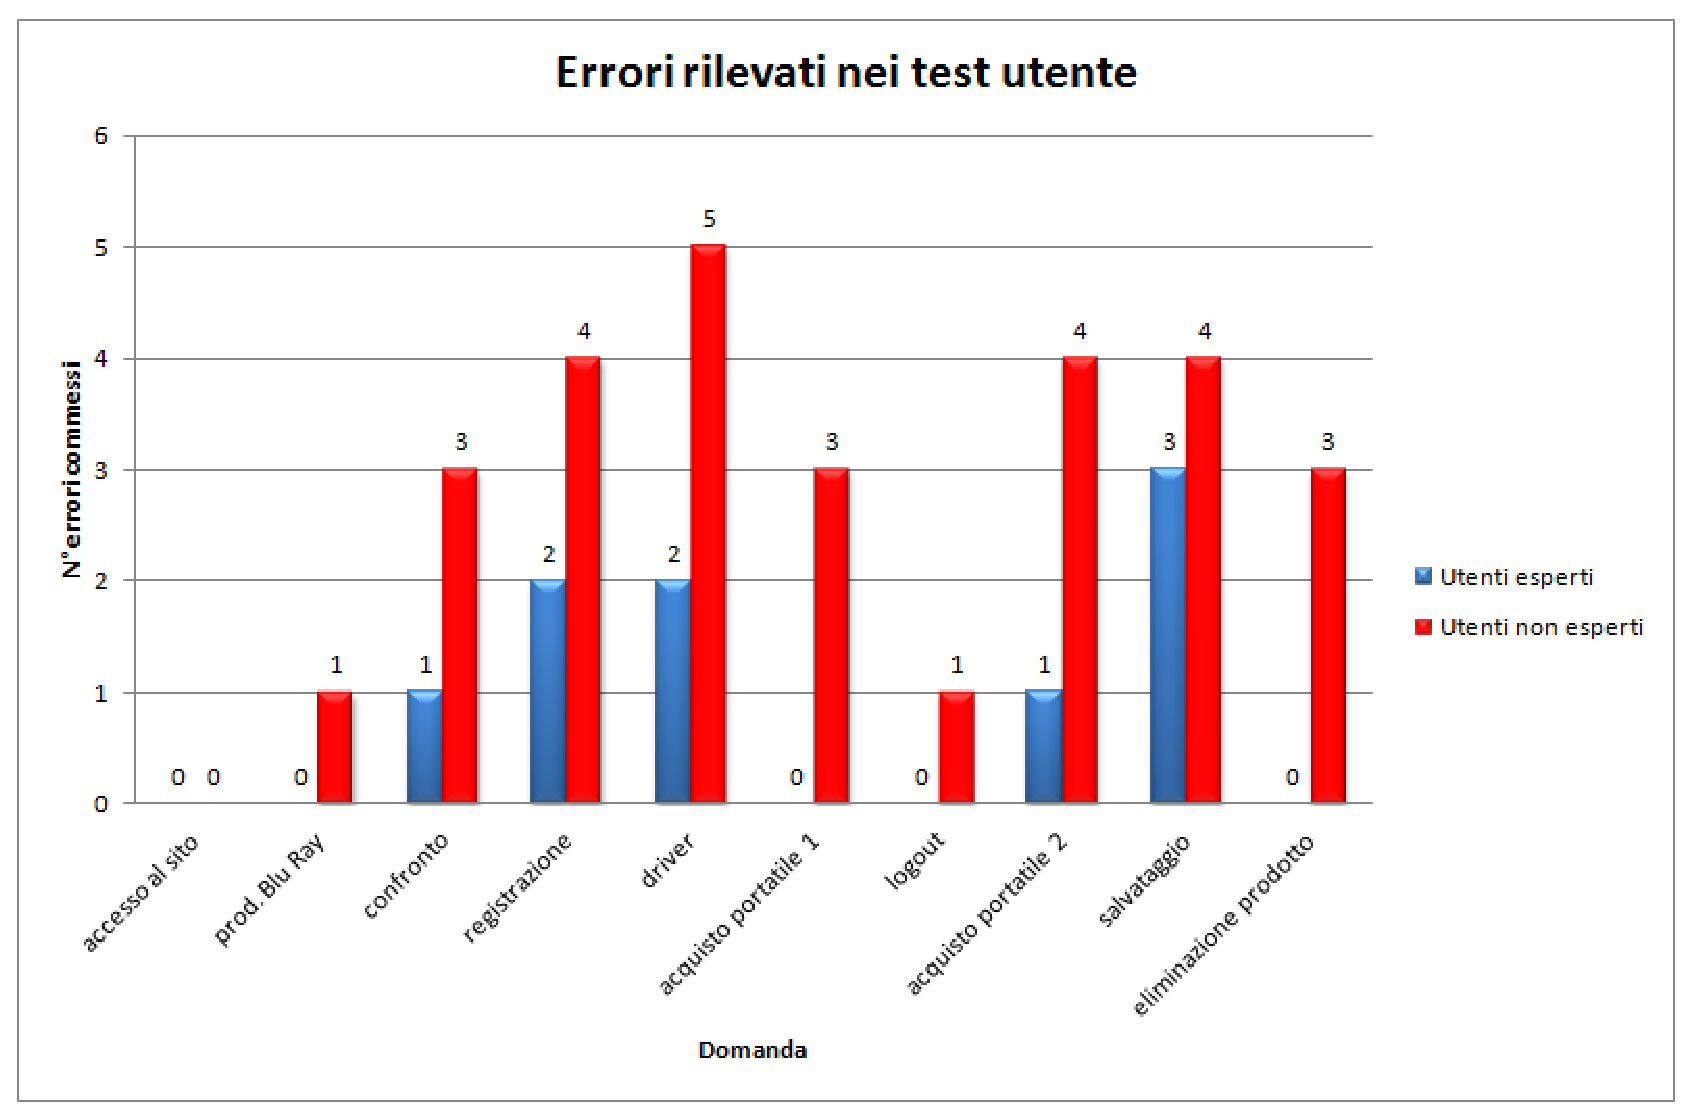
\includegraphics[angle=90, scale=0.75]{figure/grafico_errori_test_utente.eps}
\caption{rafico riportante il numero di errori commessi dagli utenti nella risoluzione dei vari task}
\label{fig:errori_test}
\end{figure}

Dal primo grafico(figura: \ref{fig:tempi_esecuzione_test}) si evince che i tempi impiegati dagli utenti non esperti siano spesso inaccettabili: la ricerca di drivers e software per il computer, cos� come la registrazione hanno comportato lo sforamento del tempo massimo. \\ 
In particolare la registrazione � stata particolarmente ostica per gli utenti non esperti, dovuta a pi� problemi sovrapposti: in primo luogo  non � immediatamente visibile alcun bottone di registrazione, portando l'utente a perdersi all'interno del sito alla ricerca di un link che mandi alla registrazione. Dopo ci� lo scoglio successivo � stata la compilazione dei vari form: ha spesso costretto a ricompilare pi� volte i campi errati, resettando i campi della password ogni iterazione, cosicch� gli utenti che avevano gi� commesso un errore (o pi� errori) hanno avuto un ulteriore rischio di sbagliare nei casi in cui la password fosse stata giusta. Infine le diciture d'errore in lingua inglese non hanno aiutato in alcun modo gli utenti che non parlano questa lingua.\\
Altra operazione che comporta notevole spreco di tempo � la configurazione dei computer da acquistare: la pagina degli acquisti per privati � piuttosto caotica, non � immediato capire che alcuni passi del wizard possono essere saltati e l'utente � portato a seguire sempre il wizard in maniera lineare; spesso anche gli utenti esperti non si sono resi conto del fatto che fossero presenti scorciatoie.\\
Talvolta anche compiti come la rimorzione di elementi dal carrello si � rivelata pi� lenta del previsto: gli utenti meno esperti hanno spesso perso tempo per cercare di cancellare il portatile dal carrello, uno ha addirittura effettuato il log-out.\\
Pi� in generale va sottolineato che gli strumenti offerti dal sito spesso sono di poco aiuto, caso eclatante � il form per la ricerca libera, il quale avrebbe dovuto velocizzare diversi task, soprattutto per i pi� esperti, purtroppo spesso i risultati delle ricerche avevano poco o nulla a che vedere con quanto desiderato dagli utenti. Un'utente esperto per ovviare al problema ha utilizzato il motore di ricerca google per effetturare ricerche all'interno del sito Dell, funzionando dove il search engine di Dell aveva fallito.
Gli help e le sezioni di aiuto non sono mai state usate da nessun utente, nemmeno dai meno esperti quando letteralmente si ``perdevano'' all'interno del sito Dell. Ci� sta ad indicare che essi hanno poca visibilit� all'interno della pagina, oppure non sono dove ci si aspetterebbe.\\
Si nota infine che gli utenti meno esperti oltre ad impiegare pi� tempo dei loro colleghi pi� abituati a navigare facciano anche pi� errori, e in alcuni casi hanno pensato di aver concluso il compito senza invece averlo portato a termine (caso del punto 9, dove era richiesto il salvataggio della configurazione).
